\appendix
\section{Condizioni al contorno aperte}
\label{appendix:nonrefl}
Dato un sistema dinamico (per semplicità in una dimensione) descritto dalle seguenti equazioni differenziali:
\begin{equation}
    \pd{\vv{U}} + \vv{A} \pdx{\vv{U}}{x} + \vv{C}= 0
    \label{eq:cont1}
\end{equation}
ed ipotizziamo di volerlo studiare nell'intervallo $a\le x \le b$ con delle condizioni al contorno per cui sono ammesse onde entranti ed uscenti, la difficoltà di questa scelta di condizione al contorno sta nel distinguere quali siano le onde entranti e quali quelle uscenti durante l'evoluzione. La soluzione di questo problema la si ottiene mediante l'uso delle equazioni caratteristiche.
\subsection{Equazioni caratteristiche}
Si possono ottenere le equazioni caratteristiche diagonalizzando la matrice $\vv{A}$ e calcolando la relativa matrice di trasformazione $\vv{S}$:
\[
    \vv{S} \vv{A} \vv{S}^{-1} = \vv{\Lambda}
\]
con $\vv{\Lambda}$ matrice diagonale avente sulla diagonale stessa gli autovalori di $\vv{A}$. \\
In particolare si può moltiplicare l'equazione \ref{eq:cont1} per $\vv{S}$ e ottenere: 
\[
    \vv{S} \pd{\vv{U}} + \vv{\Lambda} \vv{S} \pdx{\vv{U}}{x} + \vv{S}\vv{C}= 0
\]
Questo sistema può essere espresso separatamente per ciascun autovalore $\lambda_i$ con $i = 1, ..., N$ e con $N$ numero di variabili del sistema 1D:
\begin{equation}
    \vv{I}_i \pd{\vv{U}} + \vv{\lambda}_i \vv{I}_i \pdx{\vv{U}}{x} + \vv{I}_i \vv{C} = 0 \label{eq:caratt}
\end{equation}
In cui $\vv{I}_i$ sono gli autovettori sinistri di $\vv{A}$
\[\vv{I}_i \vv{A} = \lambda_i \vv{I}_i\]
L'equazione \ref{eq:caratt} è definita come l'equazione caratteristica di quella di partenza. Il vantaggio di esprimere il sistema in termini delle caratteristiche è che risulta evidente dal segno dei $\lambda_i$ quali siano le onde che propagano nell'una o nell'altra direzione, infatti se definiamo la quantità $\vv{V}$ come:
\[
    dV_i = \vv{I}_id\vv{U} + \vv{I}_i \vv{C}dt
\]
Si ha subito che l'equazione \ref{eq:caratt} può essere espressa in forma di semplice advezione:
\[
    \pd{V_i} + \lambda_i \pdx{V_i}{x} = 0
\]
in questo modo è possibile discriminare tra le condizioni al bordo nel caso di onda uscente o entrante. \\
\subsection{Condizione al bordo non riflettente di Hedstrom}
Le condizioni al bordo non riflettenti di Hedstrom possono essere riassunte nella seguente:
\begin{center}
    \textit{L'ampiezza delle onde entranti è costante nel tempo ai bordi.}
\end{center}
Matematicamente, se $V_i$ è l'ampiezza di un'onda entrante si ha che:
\[
    \left. \frac{d}{dt} V_i\right|_{x = a, b} = 0 
\]
Quindi in termini delle equazioni caratteristiche possiamo dire che, se un'onda è entrante:
\begin{equation}
    \left. \left(\vv{I}_i \pd{ \vv{U}} + \vv{I}_i \vv{C}\right)\right|_{x = a, b} = 0 
\end{equation}
mentre se l'onda è uscente è possibile utilizzare l'equazione \ref{eq:caratt} per la sua evoluzione ai bordi. Si può risassumere la formulazione di queste condizioni al contorno con la seguente equazione:
\begin{equation}
    \left.\left(\vv{I}_i \pd{\vv{U}} + \Lagr_i + \vv{I}_i\vv{C} \right)\right|_{x = a, b}= 0 
	\qquad \mbox{con} \qquad 
    \begin{dcases}
	\Lagr_i = \lambda_i\vv{I}_i \pdx{\vv{U}}{x} & \mbox{Per onde uscenti}\\
	\Lagr_i = 0 & \mbox{Per onde entranti}
    \end{dcases}
    \label{eq:caratt_final}
\end{equation}

\subsection{Applicazione al caso MHD in analisi}
Partiamo dal sistema di equazioni \ref{eq:init_elsa1}, \ref{eq:init_elsa2} (quindi prima di esprimerlo in termini di variabili di Elsasser), tale sistema può essere espresso come la \ref{eq:cont1}:
\[
    \vv{U} = \begin{pmatrix} u \\ b \end{pmatrix} 
    \qquad \vv{A} = \begin{pmatrix} u & -1 - b \\ -1-b & u\end{pmatrix} 
\]
Come termine $\vv{C}$ si prende il termine diffusivo che appare nelle equazione per $b$:
\[
    \vv{C} = \begin{pmatrix} 0 \\ -R_m^{-1} \frac{\partial^2}{\partial x^2} b  \end{pmatrix}
\]
Si ottengono subito gli autovalori e gli autovettori sinistri di $\vv{A}$:
\begin{align*}
    &\lambda_1 = -1-b+u     && \vv{I}_1 = \begin{pmatrix} 1 \\ 1 \end{pmatrix}\\
    &\lambda_2 = 1+b+u     && \vv{I}_2 = \begin{pmatrix} 1 \\ -1 \end{pmatrix}
\end{align*}
E le equazioni lungo le caratteristiche si ottengono semplicemente applicando la \ref{eq:caratt_final}:
\begin{align*}
    & \pd{u} + \pd{b} + \Lagr_1 = 0\\
    & \pd{u} - \pd{b} + \Lagr_2 - R_m^{-1} \frac{\partial^2}{\partial x^2} b = 0\\
\end{align*}
In cui i termini $\Lagr_i$ vanno definiti in modo distinto per il bordo destro e sinistro esplicitiamo solo $\Lagr_1$ e partiamo dal bordo sinistro: 
\[
    \begin{dcases}
	\Lagr_1 = (-1+u-b)\left(\pdx{u}{x} + \pdx{b}{x}\right) & -1 + u - b > 0\\
	\Lagr_1 = 0 & -1 + u - b < 0\\
    \end{dcases}
\]
Si sottointende che tutte le quantità sono calcolate nel bordo sinistro, quindi in $a$. Per il bordo destro si ha l'esatto opposto:
\[
    \begin{dcases}
	\Lagr_1 = 0 & -1 + u - b > 0\\
	\Lagr_1 = (-1+u-b)\left(\pdx{u}{x} + \pdx{b}{x}\right) & -1 + u - b < 0\\
    \end{dcases}
\]
Quindi è possibile ricavare sui bordi la somma e la differenza delle derivate temporali di $u$ e $b$, di conseguenza risulta nota anche la derivata temporale delle singole variabili.\\
Si nota tuttavia che le equazioni caratteristiche equivalgono proprio a scrivere il sistema in termini di variabili di Elsasser, è facile quindi vedere che la condizione di Hedstrom agisce direttamente in termini di $Z^{\pm}$. Per questo motivo il sistema è stato studiato in termini queste variabili anziché $u$ e $b$.
\section{Filtro di Lele}
Si utilizza un filtro di Lele per controllare i fenomeni non lineari nei punti in cui le soluzioni $Z^{\pm}$ generano dei gradienti molto forti. In tali punti possono generarsi delle perturbazioni numeriche che, propagando, interagiscono non linearmente con le soluzioni stesse creando instabilità numerica. 
La peculiarità di questi filtri è quella abbattere le onde a frequenza prossima a quella di Nyquist e di rallentarne la loro propagazione. \\
Dato un segnale $f$ il suo segnale filtrato $\hat{f}$ può essere costruito a partire da una espressione alle differenze finite:
\begin{equation}
    \beta \hat{f}_{i-2} + \alpha \hat{f}_{i-1} +\hat{ f}_i + \alpha\hat{ f}_{i+1} + \beta f_{i+2} = 
    a f_i + \frac{d}{2} \left(f_{i+3} + f_{i-3} \right) + \frac{c}{2} \left(f_{i+2} + f_{i-2} \right) + \frac{b}{2} \left(f_{i+1} + f_{i-1} \right)
    \label{eq:lelefilter}
\end{equation}
Questa equazione è implicita, la soluzione si ottiene invertendo la matrice pentadiagonale associata al sistema.\\
Si analizza l'espressione in trasformata di fourier, la simmetria spaziale dei termini in gioco (presenti sempre in forma $f_{i+n} + f_{i-n}$) è utile a rendere reale la funzione di trasferimento (la parte immaginaria dei termini $e^{ni\Delta x} + e^{-ni\Delta x}$ si annulla):
\[
    T(\omega) = \frac{a + b \cos (\omega) + c \cos(\omega) + d \sin(\omega)}{ 1 + 2\alpha\cos(\omega) + 2\beta\cos(\omega)}
\]
A questo punto per costruire un filtro a partire dalla \ref{eq:lelefilter} basta richiedere che per la frequenza di Nyquist $\omega = \pi$ la funzione di trasferimento sia nulla (per questo tipo di schemi tale richiesta comporta anche l'annullamento della derivata prima di $T(\omega)$ in $\pi$), inoltre bisogna imporre il passaggio delle basse frequenze quindi $T(0) = 1$.\\
Vista la quantità di parametri liberi è possibile richiedere anche che la $T(\omega)$ sia "liscia" in $\omega = \pi$, da qui emergono le due ulteriori condizioni usate da Lele:
\[
    \frac{d^2T}{d\omega^2}(\pi) = 0  \qquad \frac{d^2T}{d\omega^4}(\pi) = 0
\]
Sviluppando in serie di Taylor le derivate e mettendo tutto a sistema si può ottenere uno schema di ordine 6 in $x$ con i coefficienti:
\begin{center}
$\alpha = 0$, $\beta = 3/10$, $a=0.5$, $b = 0.75$, $c = 3/10$, $d = 1/20$.
\end{center}
Essendo uno schema per cui il punto $i$ viene valutato tramite i suoi limitrofi è necessario trattare i bordi separatamente, la soluzione proposta da Lele è utilizzare uno schema esplicito per i 3 punti estremali destri e sinistri:
\begin{align*}
    &\hat{f}_1 = \frac{15}{16} f_1 + \frac{1}{16}\left(4f_2 - 6f_3 + 4f_4 - 5f_5 \right)\\
    &\hat{f}_2 = \frac{3}{4} f_2 + \frac{1}{16}\left( f_1 + 6f_3 - 4f_4 + f_5\right)\\
    &\hat{f}_3 = \frac{5}{8} f_2 + \frac{1}{16}\left(-f_1 + 4f_2 + 4_f4 - f_5 \right)
\end{align*}
Tale schema ai bordi è di ordine 4 in $x$ e garantisce una chiusura per lo schema \ref{eq:lelefilter} nel caso di condizioni al contorno non riflettenti.
\subsection{Test del filtro}
Si può testare il filtro prendendo un segnale gaussiano in una griglia finita, la $\sigma$ di tale segnale viene scelta in modo da eccitare tutti i modi esprimibili nella griglia. Si è scelto quindi $\sigma = 2 dx$ e $\mu = L/2$.\\
Si applica successivamente il filtro di cui sopra sul segnale gaussiano e si osserva la sua azione sulla trasformata di Fourier del segnale. 
Si riporta il risultato ottenuto in Figura \ref{fig:lele}, compatibile con quanto ottenuto da Lele nel suo articolo per il filtro in questione.
La funzione riportata nel secondo grafico di Figura \ref{fig:lele} è l'attenuazione dei modi così definita:
\[
    G(k) \equiv \frac{f_k^{fin}}{f_k^{in}}
\]
\begin{figure}[H]
    \centering
    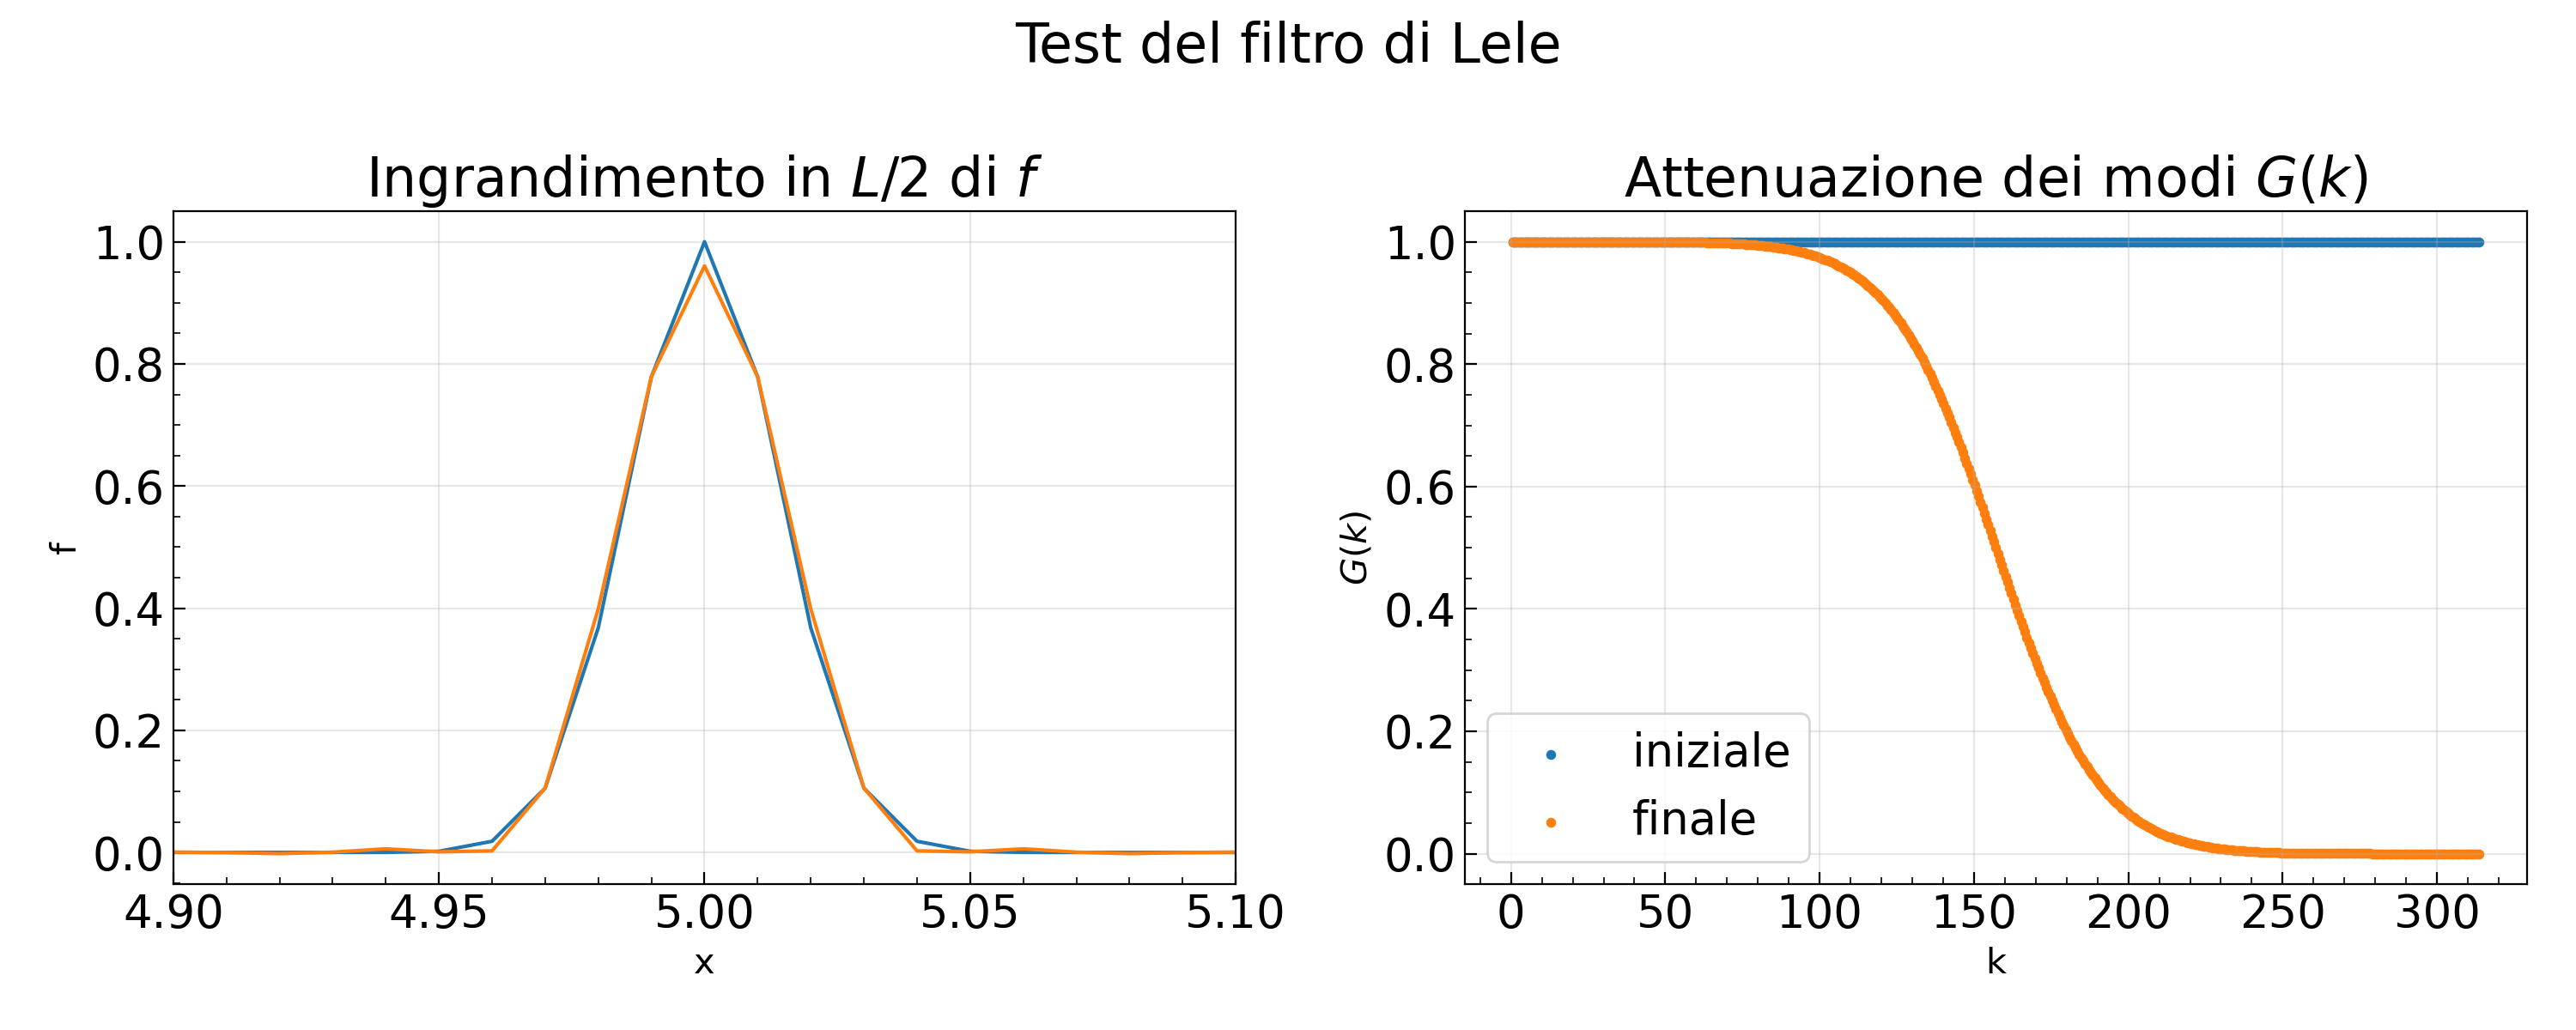
\includegraphics[width=\textwidth]{../../figure/test_lelefilter.png}
    \caption{\scriptsize Test del filtro di Lele con condizione iniziale Gaussiana}
    \label{fig:lele}
\end{figure}

